Model Predictive Control (MPC), it is an optimal control technique where the actions are chosen solving an optimization problem, composed by a set of constraints and an
objective function to be minimized over a finite horizon.
\begin{align}
    \min_{u(0), u(1), \dots, u(N-1)} \quad & \sum_{k=0}^{N-1} \ell(x(k), u(k)) + \ell_f(x(N)) \\
    \text{s.t.} \quad & x(k+1) = f(x(k), u(k)), \quad k = 0, \dots, N-1, \\
    & x(k) \in \mathcal{X}, \quad u(k) \in \mathcal{U}, \quad k = 0, \dots, N-1, \\
    & x(0) = x_{\text{0}}
\end{align}
Here, $\mathcal{U}$ and $\mathcal{X}$ denote the admissible sets for inputs and states, respectively, while $x_{\text{0}}$ is the initial state.
One of the main advantages of this control approach is the ability to handle multivariable interactions and constraints. However, solving the above optimization problem in real time can be computationally challenging, especially for large-scale or highly nonlinear systems. This is one reason why neural networks have been employed to either approximate the system model or enhance the optimization process. In our case, we have used Neural Networks to predict the next state after the application of the control input given by the MPC.

\subsection{Cost function}
Our objective is to minimize at each step the error with respect to the reference 
trajectory, both in translational and rotational dimension, while also maintaining the
module of the input actions as low as possible. A terminal state term is present too,
where the translational and rotational errors of the last horizon step are tried to 
be minimized. Thus, the cost function is composed by the following three terms:
\begin{enumerate}
    \item \textbf{Spatial error}: at each step of the horizon, the squared errors over the state variables are summed together
                                  \begin{equation}
                                      J_{sp_{k}} = W_{x} \sum_{i=0}^{n}x_{i_{k}}^2
                                  \end{equation}
                                  where $x_{i_{k}}$ it is the $i$-th component of the state vector at the $k$-th instant.

    \item \textbf{Terminal state}: to make sure the final state over the horizon is good, we add a related penalty term in the terminal state $N$:
                                   \begin{equation}
                                    J_{sp_{N}} = W_{x} \sum_{i=0}^{n}x_{i_{N}}^2
                                   \end{equation}
                                   where $x_{i_{k}}$ it is the $i$-th component of the state vector at the last instant over the horizon
    \item \textbf{Input}: it penalizes high magnitudes of input controls 
                                   \begin{equation}
                                        J_{u_{k}} = W_{u} \sum_{i=0}^{n}u_{i_{k}}^2
                                   \end{equation}
                                   where $u_{i_{k}}$ it is the $i$-th component of the control vector at the $k$-th instant.
                               

\end{enumerate}

\subsection{Constraints}
The constraints of the NLP concerns some limitations on the state of the vehicle model 
and on the dynamics of the system. 
In detail, we have just two constraints:
\begin{enumerate}
    \item \textbf{Initial state}: the initial state of the unicycle model must be the current measured state. 
                                  Therefore, defining the vehicle state as $x$:
                                  \begin{equation}
                                    x_0 = x_{current}
                                  \end{equation}
    \item \textbf{Dynamics}: given the robot state at a certain time-step as $x_t$, an input at the same time-step as $u_t$
                             and the dynamic model of the system defined as $\text{f}_\text{expl}$, 
                             we establish that the next state is obtained by applying the input at the given state according to
                             dynamic model:
                             \begin{equation}
                                x_{t+1} = \text{f}_\text{expl}(x_t, u_t)
                             \end{equation} 
\end{enumerate}

\subsection{Unicycle}
For our formulation, we have considered a discrete-time version of the model equations (\ref{eq:unicycle}) obtained via Euler integration:
\begin{align}
    \label{eq:unicycle_euler}
    \begin{cases}
        x_{k+1} = x_{k} + T_s\, v_{k} \cos \theta_{k}, \\
        y_{k+1} = y_{k} + T_s\, v_{k} \sin \theta_{k}, \\
        \theta_{k+1} = \theta_{k} + T_s\, \omega_{k}.
    \end{cases}
\end{align}
According to this, the cost function terms are the following ones:
\begin{enumerate}
    \item \textbf{Spatial error}: at each step of the horizon, the squared errors along x-axis, y-axis and error of orientation 
                                  are summed together
                                  \begin{equation}
                                      J_{sp} = W_{e_x} e_{x}^2 + W_{e_y} e_{y}^2 + W_{e_{\theta}} e_{\theta}^2
                                  \end{equation}
                                  where 
                                  \begin{subequations}
                                    \begin{eqnarray}
                                        e_x &=& x - x_{ref} \\
                                        e_y &=& y - y_{ref} \\
                                        e_\theta &=& \theta - \theta_{ref}
                                    \end{eqnarray}
                                  \end{subequations}

    \item \textbf{Terminal state}: to make sure the final stage is a good one, we add a penalty on errors along x-axis, y-axis and error of orientation
                                   in the terminal state
                                   \begin{equation}
                                        J_{term} = W_{e_{x_{N}}} e_{x_{N}}^2 + W_{e_{y_{N}}} e_{y_{N}}^2 + W_{e_{{\theta}_{N}}} e_{{\theta}_{N}}^2
                                   \end{equation}

    \item \textbf{Input}: it penalizes high values of input controls 
                                   \begin{equation}
                                        J_{u} = W_{v} v^2 + W_{\omega}  \omega^2
                                   \end{equation}                      
                                \end{enumerate}  

\subsection{Quadrotor}
Our work is based on a Crazyflie, which is a versatile open source
quadrotor that only weighs 27g and fits in the palm of your hand. This
particular quadrotor is characterized by a firmware that takes as inputs
roll, pitch and yaw desired poses instead of control torques. This happens
because there is a low level attitude controller which performs this
mapping for us. As a consequence, we have used a first order dynamic model
for the MPC formulation, as in \cite{crazysim}.
\begin{align}
    \label{eq:uav_first_order}
    \begin{cases}
        \dot{x} = v_{x} \\
        \dot{y} = v_{y} \\
        \dot{z} = v_{z} \\
        \dot{v}_{x} = -(\cos\psi \sin\theta \cos\phi + \sin\psi \sin\phi) \frac{T}{m}\\
        \dot{v}_{y} = -(\sin\psi \sin\theta \cos\phi - \cos\psi \sin\phi) \frac{T}{m} \\
        \dot{v}_{z} = -(\cos\theta \cos\phi) \frac{T}{m} +g\\
        \dot{\phi} = \frac{\phi_c - \phi}{\tau}\\
        \dot{\theta} = \frac{\theta_c - \theta}{\tau}\\
        \dot{\psi} = \frac{\psi_c - \psi}{\tau}\\ 
    \end{cases}  
\end{align}
In this models the state is composed by the cartesian position, the cartesian velocities and the roll pitch yaw angles.

\begin{align}
    \label{eq:state_uav}
        \mathcal{X} &= \begin{bmatrix}x & y & z & v_x & v_y & v_z & \phi & \theta & \psi \end{bmatrix}^T \\
        \label{eq:control_uav}
\end{align}

The output of the MPC is the desired roll, pitch and yaw angles, which are
then sent to the low level attitude controller of the Crazyflie, as shown in figure \ref{fig:quadrotor_mpc}.

\begin{figure}[H]
    \centering
    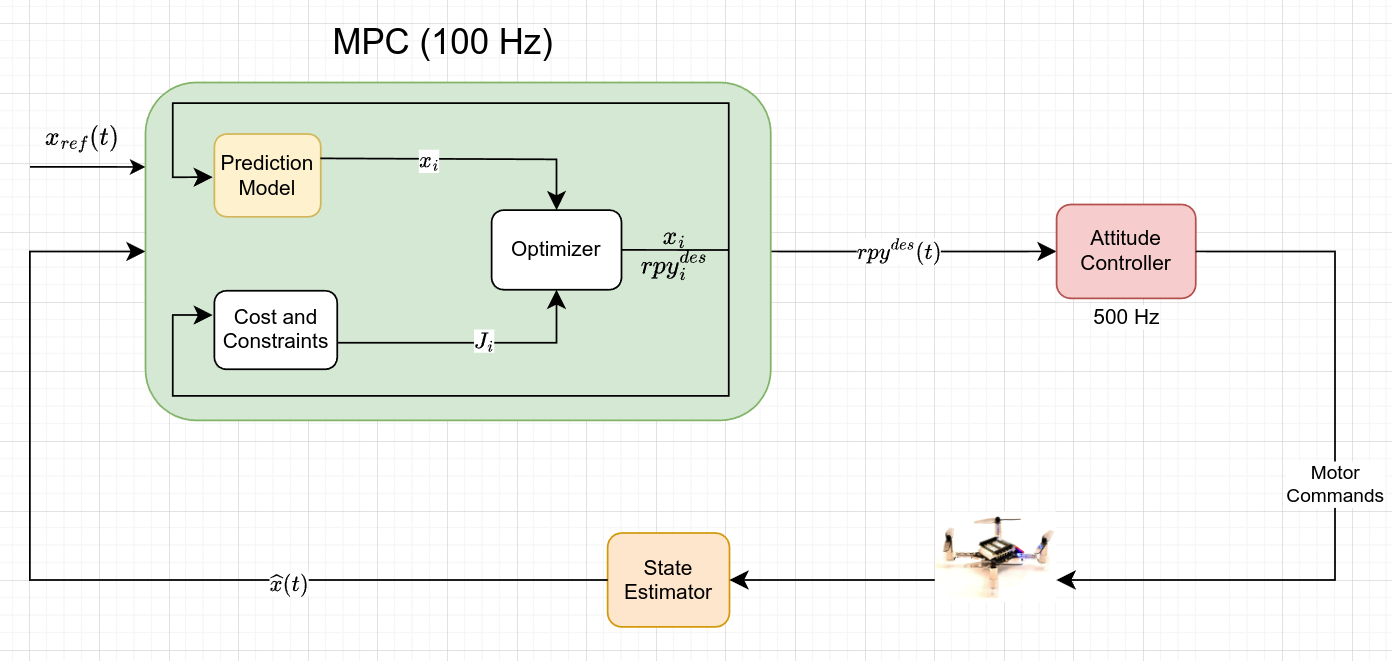
\includegraphics[width=0.8\textwidth]{assets/mpc_control_loop.png}
    \caption{MPC control scheme for the quadrotor}
    \label{fig:quadrotor_mpc}
\end{figure}

The main difference to the traditional MPC scheme lies in the prediction model (yellow box), as summarized in figure \ref{fig:mpc_comparison}.

\begin{figure}[H]
    \centering
    \begin{subfigure}{\textwidth}
        \centering
        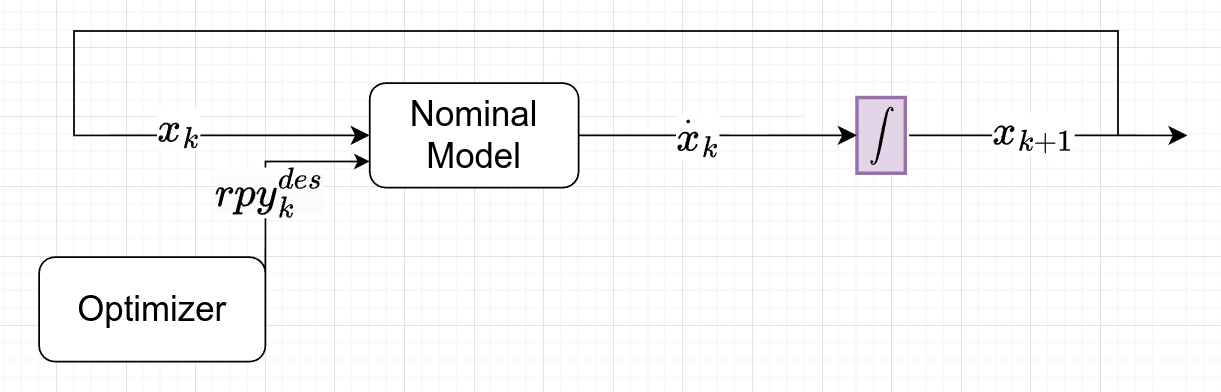
\includegraphics[width=0.8\textwidth]{assets/nominal_model_structure.png}
        \caption{Nominal model scheme}
    \end{subfigure}
    \begin{subfigure}{\textwidth}
        \centering
        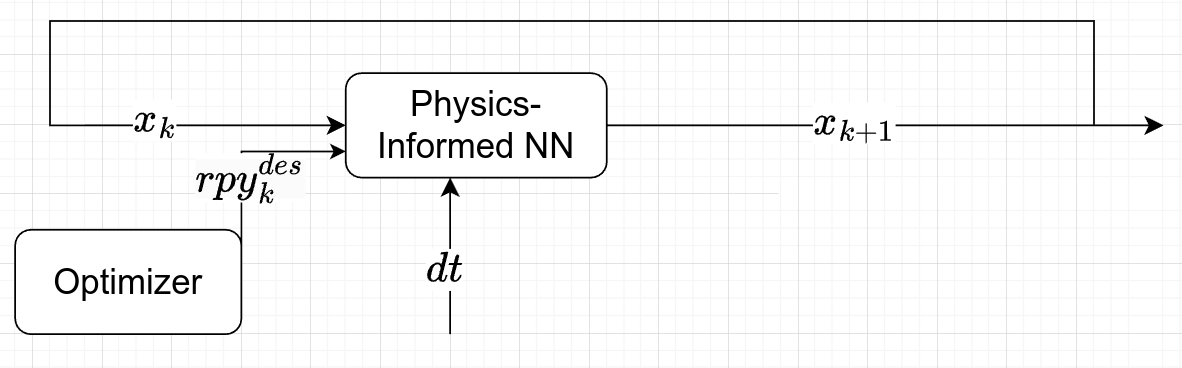
\includegraphics[width=0.8\textwidth]{assets/pinn_structure.png}
        \caption{Neural model scheme}
    \end{subfigure}
    \caption{Comparison between traditional and neural model schemes}
    \label{fig:mpc_comparison}
\end{figure}

\newpage
